\paragraph{QuizziPedia::Front-End::Directives::SubscribeResultDirective}

\label{QuizziPedia::Front-End::Directives::SubscribeResultDirective}

\begin{figure}[h]
	\centering
	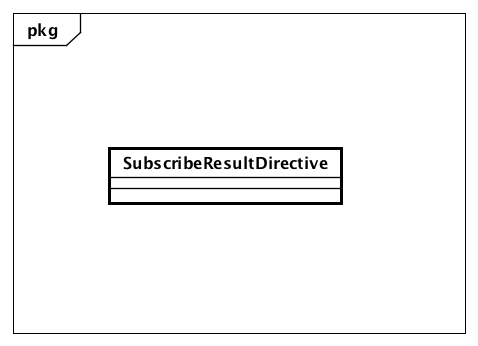
\includegraphics[scale=0.80,keepaspectratio]{UML/Classi/Front-End/QuizziPedia_Front-end_Directives_SubscribeResultDirective.png}
	\caption{QuizziPedia::Front-End::Directives::SubscribeResultDirective}
\end{figure}

\begin{itemize}
	\item \textbf{Descrizione}: directive che permette di visualizzare e iscriversi ai questionari ricercati;
	\item \textbf{Utilizzo}: permette di visualizzare e iscriversi ai questionari ricercati. Include un pulsate per ogni questionario che permette l'iscrizione ad esso.
	\item \textbf{Relazioni con altre classi}:
	\begin{itemize}
		\item \textit{IN} \texttt{ResultsView}: view contenente i risultati della ricerca effettuata, sia gli utenti che i questionari.
	\end{itemize}
	\item \textbf{Attributi}:
	\begin{itemize}
		\item \texttt{+ questionnaireDetails: Object} \\ Oggetto contenente i seguenti campi dati: \texttt{name}, \texttt{author}, \texttt{topic} e \texttt{keywords};
		\item \texttt{+ registrationButton: String} \\ Attributo che viene utilizzato per visualizzare la giusta traduzione della \textit{label\ped{G}} per il bottone di iscrizione al questionario, in italiano o in inglese;
		\item \texttt{+ controller: String} \\ Stringa contenente il nome del controller della direttiva;
		\item \texttt{+ restrict: String}: stringa che permette di definire le modalità di inserimento della direttiva all'interno della pagina;
		\item \texttt{+ scope: Scope}: oggetto scope interno della direttiva, contiene le funzionalità per gestire i dati presenti all'interno;
		\item \texttt{+ templateUrl: String}: stringa contenente il percorso del file \textit{HTML\ped{G}} che contiene la direttive.
	\end{itemize}
\end{itemize}